\let\negmedspace\undefined
\let\negthickspace\undefined
\documentclass[journal,12pt,onecolumn,article]{IEEEtran}
\usepackage{cite}
\usepackage{color,soul}
\usepackage{amsmath,amssymb,amsfonts,amsthm}
\usepackage{algorithmic}
\usepackage{float}
\usepackage{graphicx}
\usepackage{textcomp}
\usepackage{xcolor}
\usepackage{txfonts}
\usepackage{listings}
\usepackage{enumitem}
\usepackage{mathtools}
\usepackage{gensymb}
\usepackage{comment}
\usepackage[breaklinks=true]{hyperref}
\usepackage{tkz-euclide} 
\usepackage{listings}
\usepackage{multicol}
\usepackage{gvv}       
\usepackage[dvipsnames]{xcolor}
\def\inputGnumericTable{}                                
\usepackage[latin1]{inputenc}                            
\usepackage{color}                                       
\usepackage{array}                                       
\usepackage{longtable}                                   
\usepackage{calc}                                        
\usepackage{multirow}                                    
\usepackage{hhline}                                      
\usepackage{ifthen}                                      
\usepackage{lscape}
\newtheorem{theorem}{Theorem}[section]
\newtheorem{problem}{Problem}
\newtheorem{proposition}{Proposition}[section]
\newtheorem{lemma}{Lemma}[section]
\newtheorem{corollary}[theorem]{Corollary}
\newtheorem{example}{Example}[section]
\newtheorem{definition}[problem]{Definition}
\newcommand{\BEQA}{\begin{eqnarray}}
\newcommand{\EEQA}{\end{eqnarray}}
\newcommand{\define}{\stackrel{\triangle}{=}}
\renewcommand{\thesection}{\arabic{section}}
\usepackage{titlesec}
\titleformat{\section}{\raggedright\normalfont\Large}{\thesection.}{1em}{}
\titleformat{\subsection}{\raggedright\normalfont\large}{\thesubsection.}{1em}{}
\theoremstyle{remark}
\newtheorem{rem}{Remark}

\title{Hardware Experiment of Digital Clock}
\author{Murra Rajesh Kumar Reddy - EE24BTECH11043}

\begin{document}

\maketitle

\section{Abstract}
This project demonstrates the implementation of a digital clock using an Arduino Uno, six seven-segment displays, and a 7447 BCD to 7-segment decoder IC. The clock displays time in HH:MM:SS format and uses multiplexing to drive the display. The system maintains accurate time and includes buttons for setting hours, minutes, and seconds.

\section{Introduction}
A digital clock is a fundamental electronic project that displays real-time information using seven-segment displays. The aim of this project is to build a simple digital clock with six seven-segment displays controlled by an Arduino Uno and a 7447 BCD to 7-segment decoder IC. The system updates the time every second and provides push buttons to adjust the time settings.

\section{Components Required}
The following components are required to build the digital clock:

\begin{enumerate}
    \item Arduino Uno (1x)
    \item 7-Segment Display (Common Anode or Common Cathode) (6x)
    \item 7447 BCD to 7-Segment Decoder IC (1x)
    \item Resistors (330Ω) (6x)
    \item Push Buttons (4x)
    \item Connecting Wires
    \item Breadboard and Power Supply
\end{enumerate}

\section{Circuit Diagram and Connections}
The Arduino controls the seven-segment displays using multiplexing. The 7447 IC converts the BCD inputs from the Arduino into corresponding seven-segment patterns.

\subsection{Arduino Pin Configuration}

\begin{table}[h]
    \centering
    \begin{tabular}{|c|c|}
        \hline
        \textbf{Arduino Pin} & \textbf{Connected To} \\
        \hline
        PD2 - PD5 & 7447 BCD Inputs (A, B, C, D) \\
        PD6, PD7 & Hour Display Control \\
        PB0, PB1 & Minute Display Control \\
        PB2, PB3 & Second Display Control \\
        PC0, PC1, PC2 & Buttons for setting time \\
        PC3 & Reset Button \\
        \hline
    \end{tabular}
    \caption{Pin Connections}
    \label{tab:pin_connections}
\end{table}
\subsection*{Circuit Diagram of Aurdino to 7447 IC}
\begin{figure}[H]
	\centering
	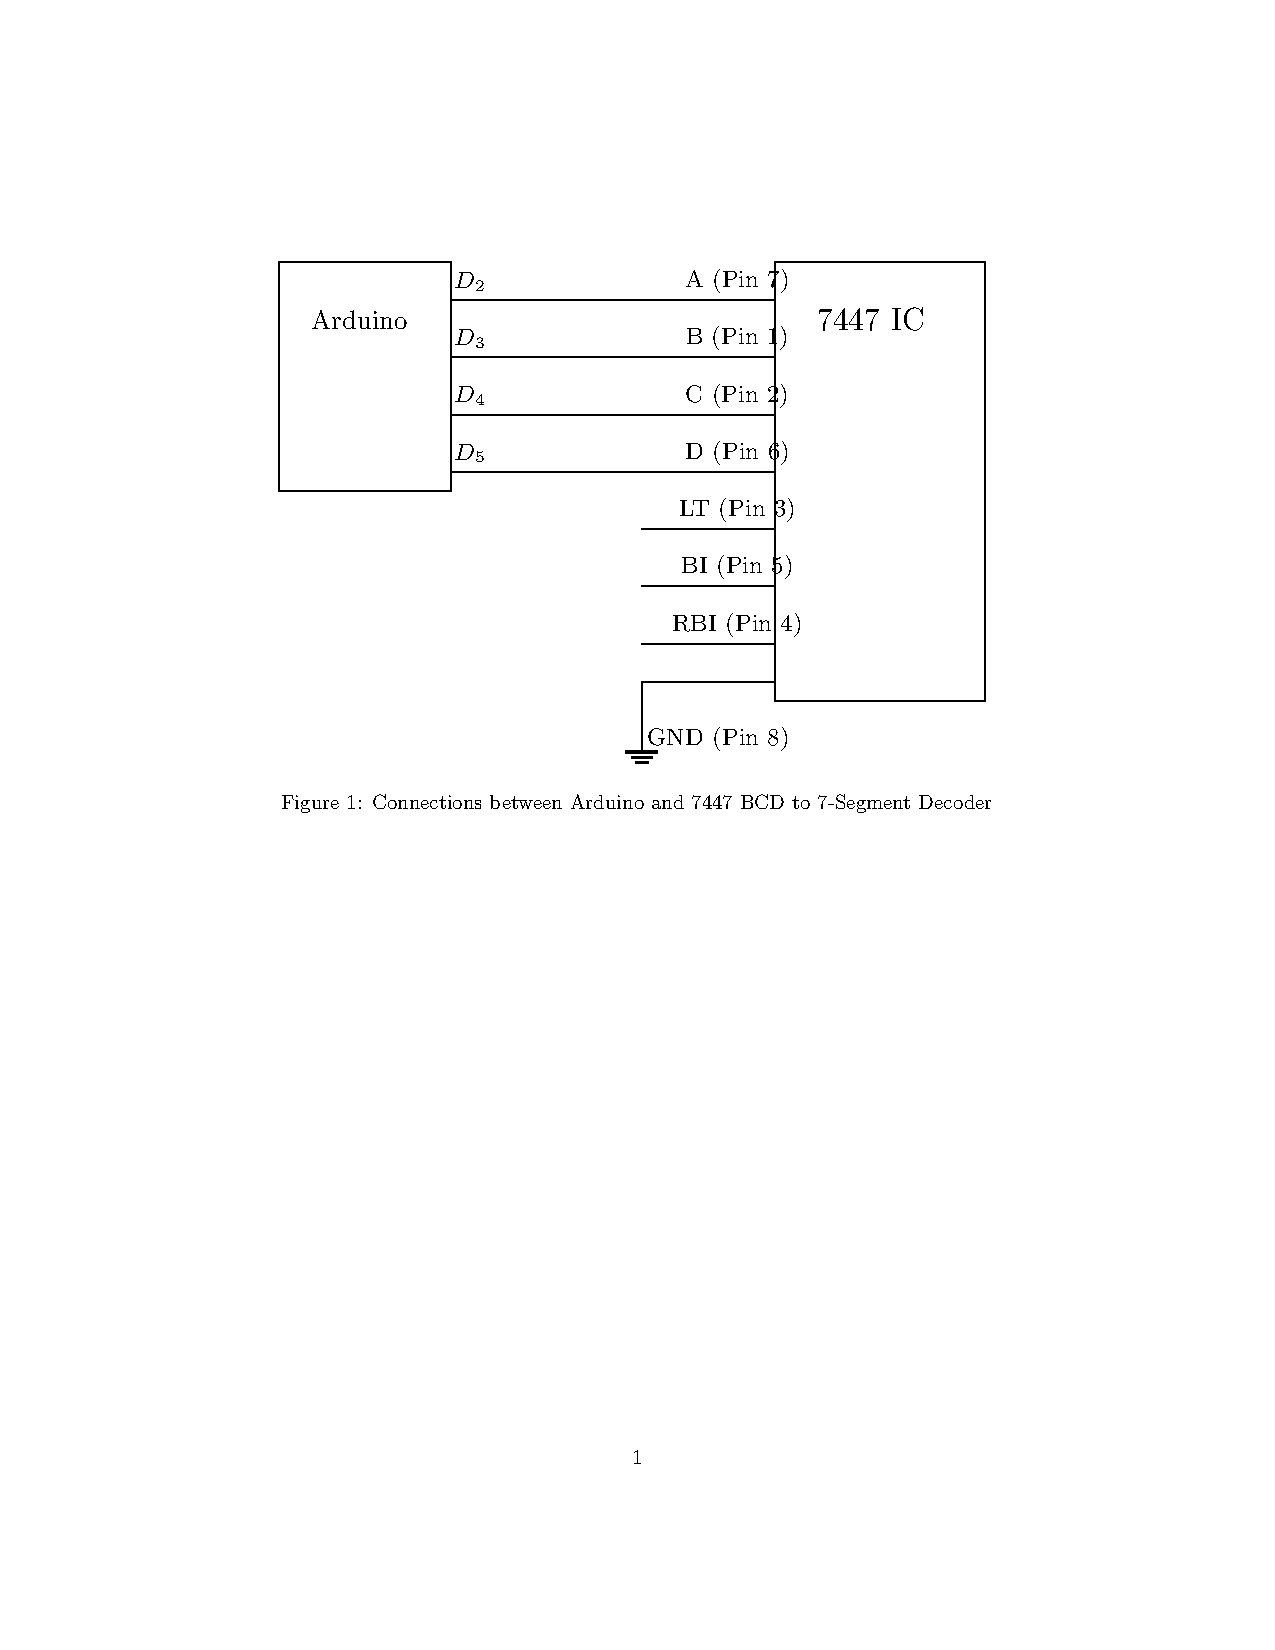
\includegraphics[width = \columnwidth]{main2.pdf}
	\label{Figure 1}
\end{figure}
\subsection{Connections from 7447 to 7-Segment Display}

\begin{table}[H]
    \centering
    \renewcommand{\arraystretch}{1.2}
    \begin{tabular}{|c|c|c|}
        \hline
        \textbf{7447 Pin} & \textbf{Function} & \textbf{7-Segment Display Pin} \\
        \hline
        13 & Segment 'a' & Connected to segment 'a' \\
        12 & Segment 'b' & Connected to segment 'b' \\
        11 & Segment 'c' & Connected to segment 'c' \\
        10 & Segment 'd' & Connected to segment 'd' \\
        9  & Segment 'e' & Connected to segment 'e' \\
        15 & Segment 'f' & Connected to segment 'f' \\
        14 & Segment 'g' & Connected to segment 'g' \\
        \hline
        Common Anode (CA) & Power for segments & Connected to VCC \\
        \hline
    \end{tabular}
    \caption{7447 to 7-Segment Display Pin Mapping}
    \label{tab:7447_connections}
\end{table}

\subsection*{Additional 7447 Pin Connections}

\begin{table}[H]
    \centering
    \renewcommand{\arraystretch}{1.2}
    \begin{tabular}{|c|c|c|}
        \hline
        \textbf{7447 Pin} & \textbf{Function} & \textbf{Connection} \\
        \hline
        16 & VCC (Power) & +5V \\
        8  & GND (Ground) & GND \\
        3  & LT (Lamp Test) & Connected to +5V (Disable Test Mode) \\
        5  & BI (Blanking Input) & Connected to +5V (Enable Display) \\
        4  & RBI (Ripple Blanking Input) & Connected to +5V (Disable Blanking) \\
        \hline
    \end{tabular}
    \caption{Additional 7447 Pin Connections}
    \label{tab:7447_additional}
\end{table}
\subsection*{Circuit Diagram of 7447 Ic to Seven segment}
\begin{figure}[H]
	\centering
	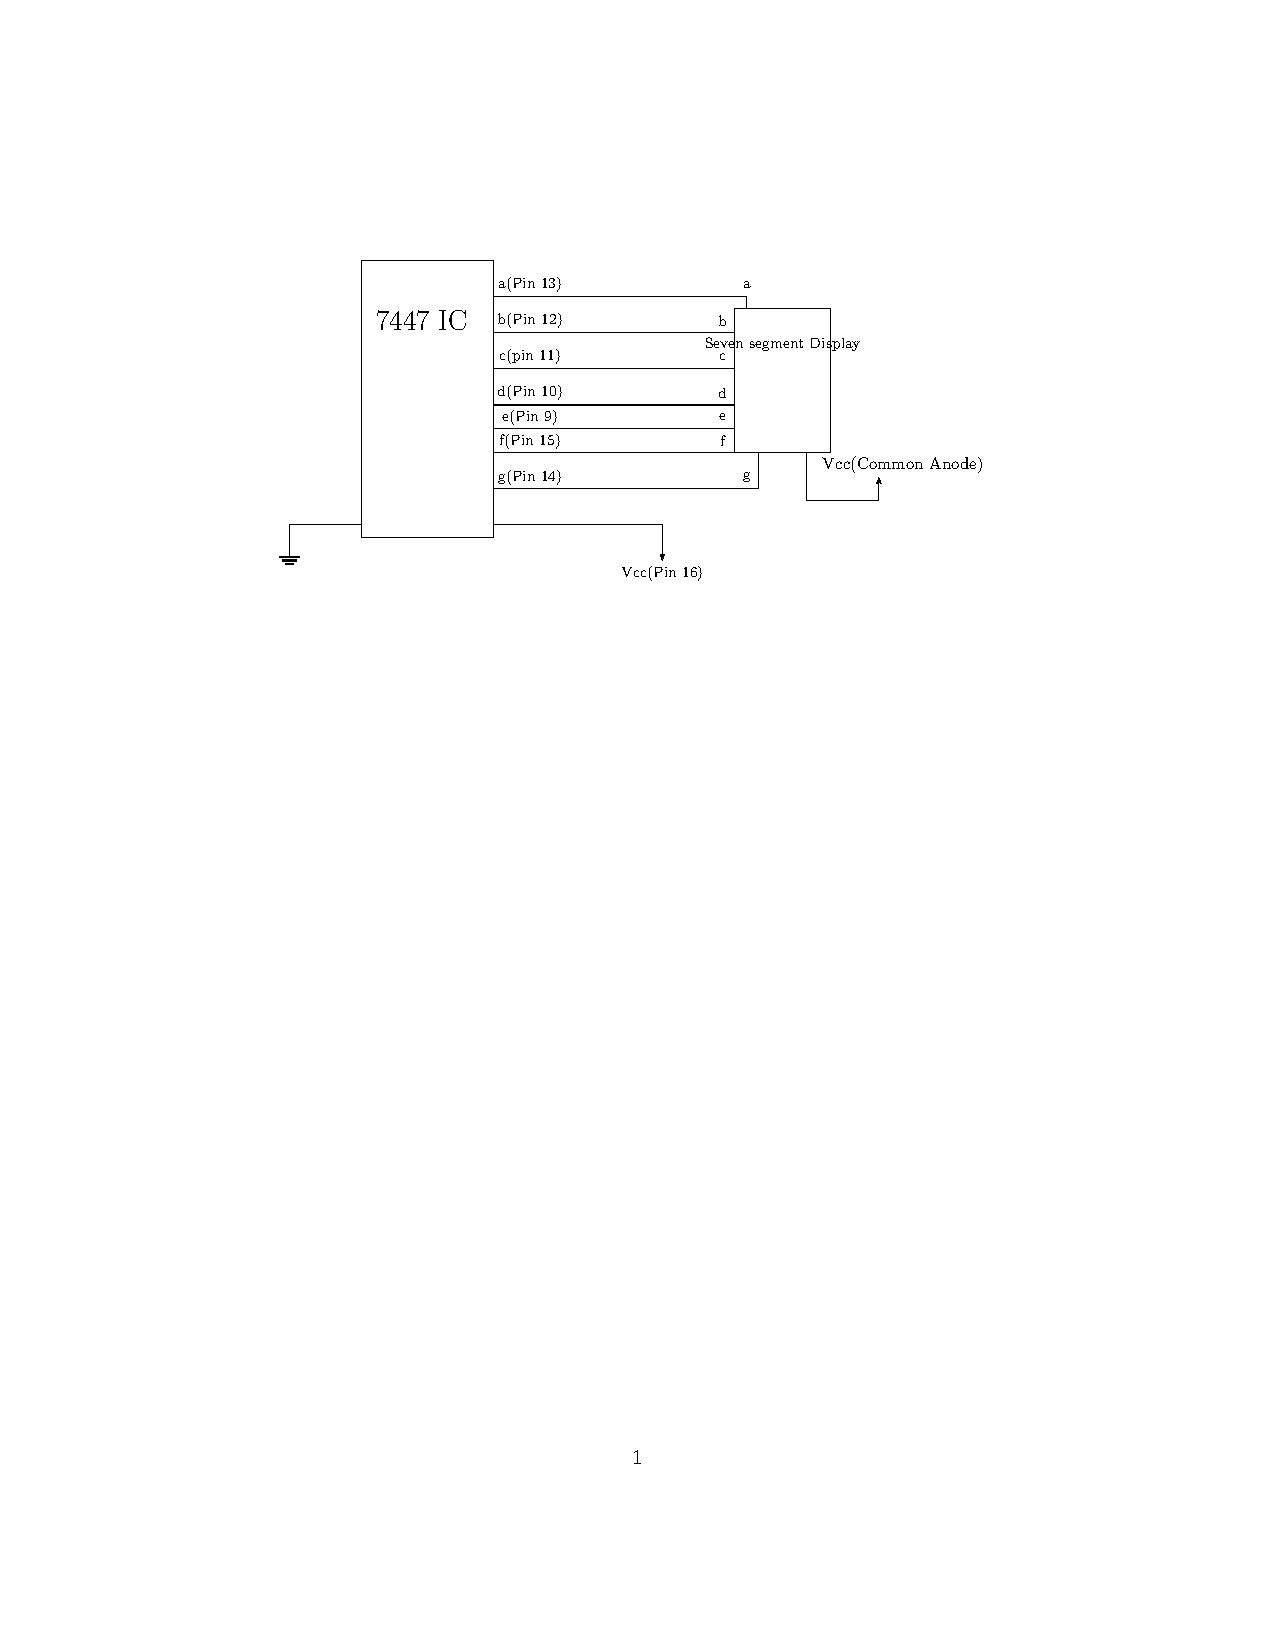
\includegraphics[width = \columnwidth]{main3.pdf}
	\label{Figure 2}
\end{figure}
\section{Code Implementation}
The following code is used to control the digital clock. The code includes functions for timekeeping, multiplexing, and handling button inputs.

\lstset{
    language=C,
    basicstyle=\ttfamily\footnotesize,
    keywordstyle=\color{blue},
    commentstyle=\color{green},
    stringstyle=\color{red},
    numbers=left,
    numberstyle=\tiny\color{gray},
    stepnumber=1,
    breaklines=true,
    frame=single
}

\begin{lstlisting}
// BCD Output Pins
#define A PD2
#define B PD3
#define C PD4
#define D PD5

// Common Display Pins
#define H1 PD6
#define H2 PD7
#define M1 PB0
#define M2 PB1
#define S1 PB2
#define S2 PB3

// Button Pins
#define SET_HOUR PC1
#define SET_MIN PC2
#define SET_SEC PC0
#define RESET_BTN PC3

// Global BCD digits for the clock
volatile uint8_t h1 = 0, h2 = 0, m1 = 0, m2 = 0, s1 = 0, s2 = 0;
volatile uint32_t millis_count = 0, last_second = 0;
uint8_t current_digit = 0;
const uint8_t mux_interval = 2;
const uint16_t debounce_interval = 200;

void init_timer0() {
    TCCR0A |= (1 << WGM01);
    TCCR0B |= (1 << CS01) | (1 << CS00);
    OCR0A = 249;
    TIMSK0 |= (1 << OCIE0A);
    sei();
}

ISR(TIMER0_COMPA_vect) {
    millis_count++;
}

uint32_t millis() {
    uint32_t ms;
    cli();
    ms = millis_count;
    sei();
    return ms;
}

uint8_t bcdIncrement(uint8_t bcd, uint8_t max) {
    if (bcd == max) return 0;
    return bcd + 1;
}

void updateTime() {
    if (millis() - last_second >= 1000) {
        last_second += 1000;
        s2 = bcdIncrement(s2, 9);
        if (s2 == 0) {
            s1 = bcdIncrement(s1, 5);
            if (s1 == 0) {
                m2 = bcdIncrement(m2, 9);
                if (m2 == 0) {
                    m1 = bcdIncrement(m1, 5);
                    if (m1 == 0) {
                        h2 = bcdIncrement(h2, 9);
                        if (h2 == 0) {
                            h1 = bcdIncrement(h1, 2);
                            if (h1 == 2 && h2 > 3) {
                                h1 = h2 = 0;
                            }
                        }
                    }
                }
            }
        }
    }
}

void setup() {
    DDRD |= 0xFC;
    DDRB |= 0x0F;
    DDRC &= ~0x0F;
    PORTC |= 0x0F;
    init_timer0();
    last_second = millis();
}

int main(void) {
    setup();
    while (1) {
        updateTime();
    }
    return 0;
}
\end{lstlisting}

\section{Results and Observations}
\begin{enumerate}
    \item The clock successfully displays real-time hours, minutes, and seconds.
    \item Time increments every second and rolls over correctly at 23:59:59.
    \item The push buttons allow manual time adjustments.
    \item The multiplexing approach ensures efficient display updates with minimal flicker.
\end{enumerate}

\section{Conclusion}
This project successfully implemented a "Digital clock" using an "Arduino Uno, six seven-segment displays, and a 7447 (BCD to 7-segment decoder) IC". The use of multiplexing allowed for efficient display control while minimizing pin usage. The system accurately keeps track of time and allows manual adjustments via push buttons. This project serves as a foundation for advanced embedded systems applications involving real-time display control.

\section{References}
\begin{enumerate}
	\item CHAT gpt
\end{enumerate}
\end{document}

